\chapter{Experimentelle Untersuchungen}
\chaptermark{Experimentelle Untersuchungen}  % short form for headlines on pages
\label{ch:EntwickelteMethode}

\section{Angewendete Methodik}
\subsection{Testumgebung}

Um die Wirksamkeit der Parallelisierung der N++-Bibliothek in C++ zu bewerten, wird ein umfassender Benchmark-Test durchgeführt. Dieser Test umfasst verschiedene Kombinationen von Threads, Anzahl an Datensätzen und verschiedenen Computern mit verschiedenen Prozessorarchitekturen, um die Auswirkungen der Implementierung auf die Leistung der Bibliothek unter unterschiedlichen Bedingungen zu untersuchen.

Das C++ Programm wurde unter Einbindung der N++-Bibliothek auf dem jeweiligen System selbst kompiliert. Dabei wurde die Optimierungsstufe O2 verwendet, welche eine für Produktionssoftware gängige Optimierungsstufe ist. Die O2 Optimierungsstufe wendet fast jede Compileroptimierung an, die die Compiler zu bieten haben. Dabei werden lediglich als sehr unsicher eingestufte Optimierungen ausgelassen. Auf Linux wurde der GCC Compiler und auf MacOS der Clang Compiler verwendet, um native Binärdateien für die spezifische Prozessorarchitektur zu kompilieren. Das heißt, das Programm wurde nicht unter Emulation sondern vollständig nativ ausgeführt.

Die Tests wird mit unterschiedlichen Thread-Anzahlen ausgeführt, darunter 10, 8, 6, 4 und 2 gleichzeitig laufenden Threads, um den Einfluss der Parallelisierung auf die Ausführungsgeschwindigkeit zu untersuchen. Zusätzlich wird das Programm auch mit einem einzelnen Thread ausgeführt, um einen Vergleich mit der vorausgegangenen Implementierung herstellen zu können. Für jede Thread-Anzahl werden außerdem verschiedene Größen an Datensätzen getestet. Die Größe der Datensätze wird über die Anzahl an Partitionen spezifiziert. Eine Partition bedeutet dabei, dass die gesamte Datenmenge verwendet wird, wohingegen 4 Partitionen bedeuten, dass nur ein Viertel, also 25\% der Datenmenge verwendet werden. Das Programm wird in diesem Test mit 1, 2, 4 und 8 Partitionen getestet, wobei es auf dem langsamsten Computer nur auf 4 und 8 beschränkt wurde.

Für jede Kombination von Threads und Partitionen werden mindestens 5 Testläufe durchgeführt, um robuste Durchschnittswerte zu erhalten und Schwankungen zu minimieren. Gemessen wird die benötigte Zeit für den gesamten Programmdurchlauf in Sekunden. Vor jedem Durchlauf werden die Testgeräte auf einen neutralen Zustand zurückgesetzt, um faire Vergleichsbedingungen sicherzustellen. Dies wird gewährleistet, indem gleiche Seeds für die Zufallszahlgeneratoren verwendet werden, und sichergestellt wird, dass keine anderen Programme laufen.
Das Ergebnis jedes Programmdurchlaufs wird in eine Datei geschrieben, um vergleichen zu können, ob mit verschiedenen Anzahlen von Threads die gleichen Ergebnisse berechnet werden.

Nach Abschluss der Testläufe werden die erzielten Ergebnisse automatisch analysiert und Durchschnittswerte für jede Kombination von Threads und Partitionen berechnet. Diese Durchschnittswerte dienen dazu, die möglichen Schwankungen der Testabläufe auszugleichen, und ein neutraleres Ergebnis zu liefern.

\subsection{Benchmark Script}

Aus 6 verschiedenen Anzahlen an Threads, 4 verschiedenen Größen der Datensätze und 5 Durchläufen pro Kombination ergeben sich 120 einzelne Tests, die pro System ausgeführt werden müssen.
Um diese Arbeit zu erleichtern und einen reproduzierbaren Testprozess zu ermöglichen habe ich ein Skript geschrieben, welches alle Tests nacheinander automatisch ausführt.

Das Skript misst die benötigten Laufzeiten der Durchläufe und schreibt nach jedem Durchlauf die benötigte Zeit in eine Datei. Zusätzlich werden die Zeit und Informationen zu jedem Durchlauf auch in eine CSV Datei geschrieben, um das Auswerten der Benchmarks auf einem System durch nur eine einzige Datei zu ermöglichen.

Als Parameter ist es möglich, die maximale Anzahl an Threads festzulegen. So ist es beispielsweise auf einem Raspberry Pi sinnvoll, das Programm nur mit maximal 4 Threads zu testen, da er nur über 4 Threads verfügt.

Das Skript ist simpel und wurde in Bash geschrieben, was die Portabilität zwischen Linux und MacOS gewährleistet. Dabei wurde jedoch das Programm bc in dem Skript verwendet, welches auf Linux standardmäßig nicht vorinstalliert ist.

\begin{figure}[H]
\begin{minted}
[
frame=lines,
framesep=2mm,
baselinestretch=1.2,
fontsize=\footnotesize,
linenos
]{bash}
#!/bin/bash
EXECUTABLE="./lucavinciguerra-bathesis"
ATTEMPTS=5
PARTITIONS=(8 4 2 1) # Partitions to be tested
THREADS=(10 8 6 4 2 1) # Thread counts to be tested
AVAILABLE_THREADS=10 # Amount of threads to be used
CSV_FILE="benchmark_results.csv"

# Run the attempt with the given values
function run_attempt {
  local threadcount=$1
  local partitioncount=$2
  local attempt=$3
  echo -e "$partitioncount partitions / $threadcount threads $attempt "
  local filename="attempt_${attempt}_${partitioncount}p_${threadcount}t.txt"
  start=$(date +%s.%3N)
  { time $EXECUTABLE > /dev/null; } 2>> "$filename"
  end=$(date +%s.%3N)
  echo "TOTAL TIME: $(echo "$end - $start" | bc) seconds" >> "$filename"
  echo "$threadcount,$partitioncount,$attempt,$(echo "$end - $start" | bc)" >> "$CSV_FILE"
}

# Run the benchmarks for all possible combinations
for partition in ${PARTITIONS[@]};do
  for threads in ${THREADS[@]};do
      if ((threads <= AVAILABLE_THREADS));then
        for ((i = 1; i <= ATTEMPTS; i++)); do
          run_attempt "$threads" "$partition" "$i"
        done
      fi
    done
done
\end{minted}
\caption{Vereinfacht dargestelltes Benchmark Skript}
\label{fig:benchmark_script_code}
\end{figure}

\section{Ergebnisse}

\subsection{Apple M1 Pro}

\begin{figure}[H]
\centering
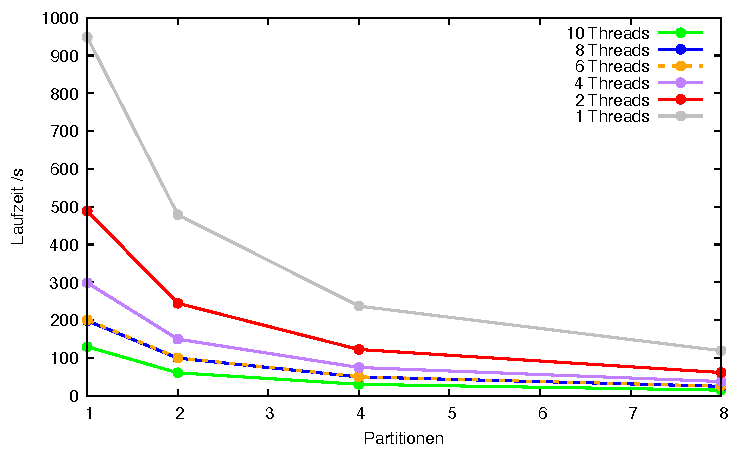
\includegraphics[width=0.8\textwidth]{../results/plots/m1pro/comp_all_threads.pdf}
\caption{Ergebnisse der Leistungstests verglichen nach Thread Anzahl}
\label{fig:m1pro_benchmark_threads}
\end{figure}

\begin{figure}[htbp!]
\centering
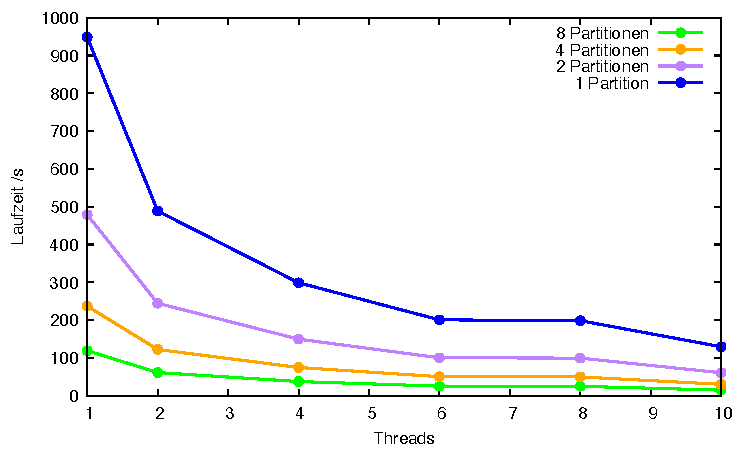
\includegraphics[width=0.8\textwidth]{../results/plots/m1pro/comp_all_partitions.pdf}
\caption{Ergebnisse der Leistungstests verglichen nach Datensatzgröße}
\label{fig:m1pro_benchmark_partitions}
\end{figure}

\subsection{AMD Ryzen 3600XT}

\begin{figure}[htbp!]
\centering
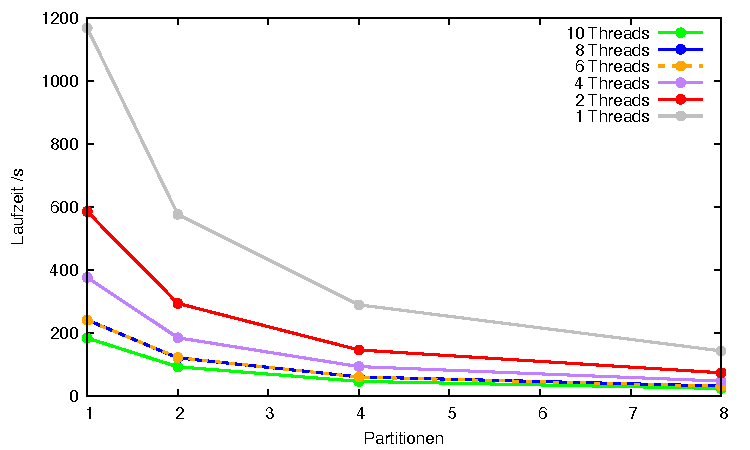
\includegraphics[width=0.8\textwidth]{../results/plots/3600xt/comp_all_threads.pdf}
\caption{Ergebnisse der Leistungstests verglichen nach Thread Anzahl}
\label{fig:ryzen_benchmark_threads}
\end{figure}

\begin{figure}[htbp!]
\centering
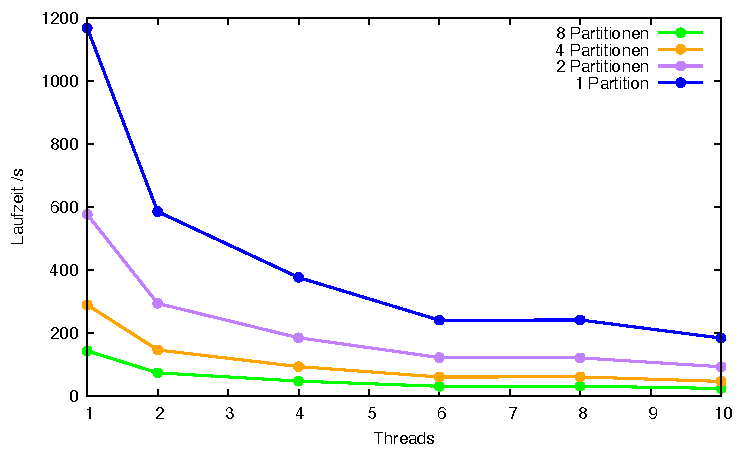
\includegraphics[width=0.8\textwidth]{../results/plots/3600xt/comp_all_partitions.pdf}
\caption{Ergebnisse der Leistungstests verglichen nach Datensatzgröße}
\label{fig:ryzen_benchmark_partitions}
\end{figure}

\subsection{Raspberry Pi 3}

\begin{figure}[htbp!]
\centering
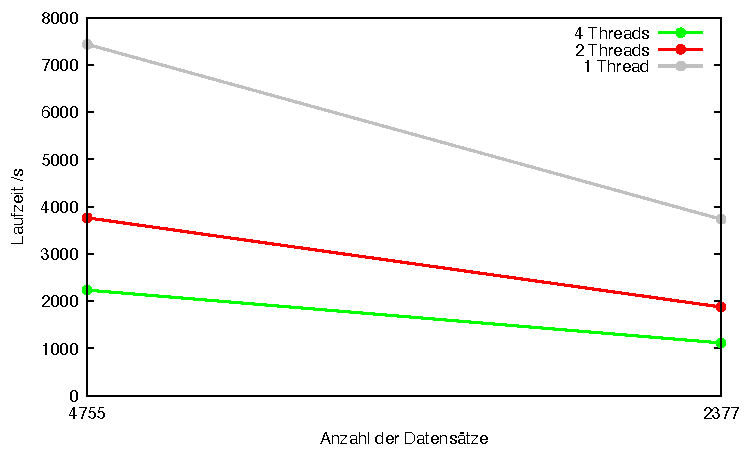
\includegraphics[width=0.8\textwidth]{../results/plots/raspberrypi3/comp_all_threads.pdf}
\caption{Ergebnisse der Leistungstests verglichen nach Thread Anzahl}
\label{fig:raspi_benchmark_threads}
\end{figure}

\begin{figure}[htbp!]
\centering
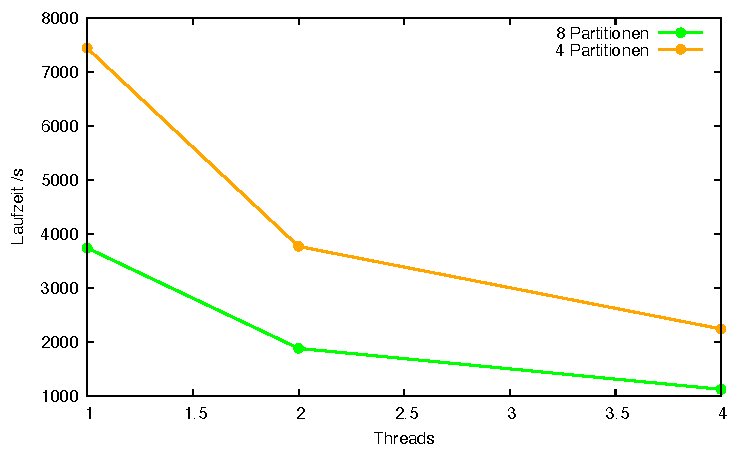
\includegraphics[width=0.8\textwidth]{../results/plots/raspberrypi3/comp_all_partitions.pdf}
\caption{Ergebnisse der Leistungstests verglichen nach Datensatzgröße}
\label{fig:raspi_benchmark_partitions}
\end{figure}

\subsection{Cloud Server}

\section{Auswertung}

\newpage
